\documentclass[border=3pt]{standalone}
\usepackage{tikz}
\usetikzlibrary{arrows.meta,calc,positioning}
\tikzset{pin/.style={-{Stealth[length=5pt]}},
  blk/.style={draw, thick, font=\sffamily\small, align=center}}
\begin{document}
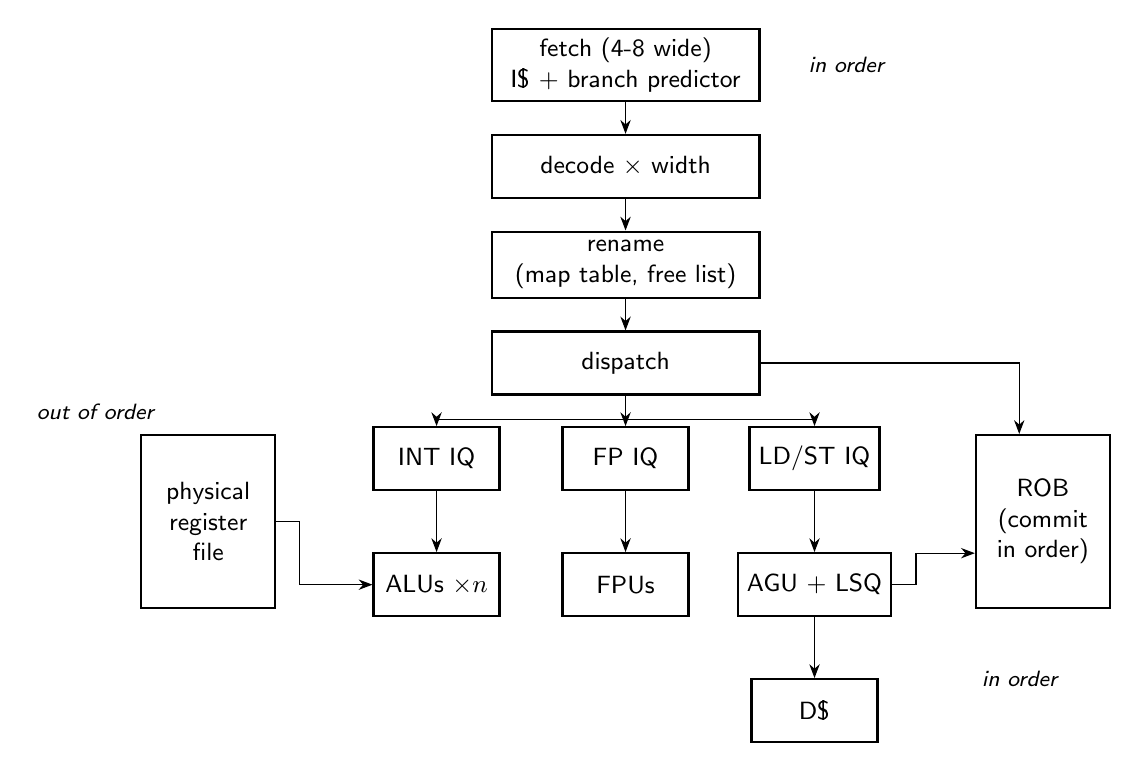
\begin{tikzpicture}[font=\sffamily\small]
  % frontend (in order)
  \node[blk, minimum width=34mm, minimum height=8mm] (fetch) at (0,0) {fetch (4-8 wide)\\I\$ + branch predictor};
  \node[blk, minimum width=34mm, minimum height=8mm, below=4mm of fetch] (dec) {decode $\times$ width};
  \node[blk, minimum width=34mm, minimum height=8mm, below=4mm of dec] (ren) {rename\\(map table, free list)};
  \node[blk, minimum width=34mm, minimum height=8mm, below=4mm of ren] (disp) {dispatch};
  \draw[pin] (fetch.south) -- (dec.north);
  \draw[pin] (dec.south) -- (ren.north);
  \draw[pin] (ren.south) -- (disp.north);
  % issue queues (out of order region)
  \node[blk, minimum width=16mm, minimum height=8mm] (iq1) at (-2.4,-5.0) {INT IQ};
  \node[blk, minimum width=16mm, minimum height=8mm] (iq2) at (0,-5.0)    {FP IQ};
  \node[blk, minimum width=16mm, minimum height=8mm] (iq3) at (2.4,-5.0)  {LD/ST IQ};
  \foreach \q in {iq1,iq2,iq3}{\draw[pin] (disp.south) -- ++(0,-3mm) -| (\q.north);}
  % execution
  \node[blk, minimum width=16mm, minimum height=8mm] (fu1) at (-2.4,-6.6) {ALUs $\times n$};
  \node[blk, minimum width=16mm, minimum height=8mm] (fu2) at (0,-6.6)    {FPUs};
  \node[blk, minimum width=16mm, minimum height=8mm] (fu3) at (2.4,-6.6)  {AGU + LSQ};
  \foreach \a/\b in {iq1/fu1, iq2/fu2, iq3/fu3}{\draw[pin] (\a.south) -- (\b.north);}
  % PRF and ROB on the sides
  \node[blk, minimum width=17mm, minimum height=22mm] (prf) at (-5.3,-5.8) {physical\\register\\file};
  \node[blk, minimum width=17mm, minimum height=22mm] (rob) at (5.3,-5.8) {ROB\\(commit\\in order)};
  \draw[pin] (prf.east) -- ++(3mm,0) |- (fu1.west);
  \draw[pin] (fu3.east) -- ++(3mm,0) |- ($(rob.west)+(0,-4mm)$);
  \draw[pin] (disp.east) -| ($(rob.north)+(-3mm,0)$);
  % D-cache
  \node[blk, minimum width=16mm, minimum height=8mm] (dc) at (2.4,-8.2) {D\$};
  \draw[pin] (fu3.south) -- (dc.north);
  % region labels
  \node[font=\sffamily\footnotesize\itshape, anchor=west] at (2.2,-0.0) {in order};
  \node[font=\sffamily\footnotesize\itshape, anchor=west] at (-7.6,-4.4) {out of order};
  \node[font=\sffamily\footnotesize\itshape, anchor=west] at (4.4,-7.8) {in order};
\end{tikzpicture}
\end{document}
